\chapter{Evaluation of Information Retrieval Systems}
\label{chap:evaluation}

\FloatBarrier
\section{Search Engine Architecture}
\label{sec:architecture}

Before diving into evaluation methodology, it is instructive to understand the high-level block diagram of a modern search engine, since each architectural component introduces measurable quality dimensions.

\begin{figure}[htbp]
\centering
\begin{tikzpicture}[
    node distance=1.1cm and 2.2cm,
    offline/.style={rectangle, rounded corners=4pt, draw=blue!70!black, fill=blue!8,
                    thick, minimum width=3.5cm, minimum height=0.9cm,
                    text width=3.4cm, align=center, font=\small},
    online/.style={rectangle, rounded corners=4pt, draw=teal!70!black, fill=teal!6,
                   thick, minimum width=3.5cm, minimum height=0.9cm,
                   text width=3.4cm, align=center, font=\small},
    index/.style={rectangle, rounded corners=4pt, draw=orange!80!black, fill=orange!9,
                  thick, minimum width=3.5cm, minimum height=0.9cm,
                  text width=3.4cm, align=center, font=\small},
    output/.style={rectangle, rounded corners=4pt, draw=green!60!black, fill=green!7,
                   thick, minimum width=3.5cm, minimum height=0.9cm,
                   text width=3.4cm, align=center, font=\small},
    arr/.style={-Stealth, thick},
    offcol/.style={arr, blue!70!black},
    oncol/.style={arr, teal!70!black},
    lbl/.style={font=\scriptsize\itshape, text=gray!70!black}
]
    %--- OFFLINE column (left) ---
    \node[offline] (dc)  at (0, 0)    {\textbf{Document Collection}\\{\scriptsize Web Crawler}};
    \node[offline, below=of dc]  (idx) {\textbf{Indexing}\\{\scriptsize Parsing · Tokeniz. · Stemming}};
    \node[index,   below=of idx] (ii)  {\textbf{Inverted Index}};

    %--- ONLINE column (right) ---
    \node[online, right=3.8cm of dc]  (q)    {\textbf{Query}\\{\scriptsize User input}};
    \node[online, below=of q]         (qp)   {\textbf{Query Processing}\\{\scriptsize Query Expansion}};
    \node[online, below=of qp]        (fe)   {\textbf{Feature Extraction}\\{\scriptsize BM25 · PageRank · CTR}};
    \node[online, below=of fe]        (lr)   {\textbf{Learned Ranking (LtR)}\\{\scriptsize LambdaMART · Neural}};
    \node[output, below=of lr]        (serp) {\textbf{SERP}\\{\scriptsize Top-10 results to user}};

    %--- Column labels ---
    \node[lbl, above=0.25cm of dc] {\textsc{Offline Phase}};
    \node[lbl, above=0.25cm of q]  {\textsc{Online Phase}};

    %--- Offline arrows ---
    \draw[offcol] (dc.south)  -- (idx.north);
    \draw[offcol] (idx.south) -- (ii.north);

    %--- Online arrows ---
    \draw[oncol] (q.south)   -- (qp.north);
    \draw[oncol] (qp.south)  -- (fe.north);
    \draw[oncol] (fe.south)  -- (lr.north);
    \draw[oncol] (lr.south)  -- (serp.north);

    %--- Inverted Index → Query Processing bridge ---
    \draw[arr, orange!80!black, dashed, thick]
        (ii.east) -- ++(0.9,0) |- (qp.west)
        node[pos=0.28, above, lbl] {candidate docs};

\end{tikzpicture}
\caption{High-level block diagram of a modern search engine: offline indexing pipeline (left) and online query processing and ranking pipeline (right).}
\label{fig:arch-en}
\end{figure}

The main components are:

\begin{itemize}
    \item \textbf{Web Crawler / Document Collection:} An automated agent that continuously discovers and downloads documents from the Web (or a closed corpus), feeding the indexing pipeline.
    \item \textbf{Parsing \& Tokenization:} Documents are linguistically analyzed: HTML is stripped, text is tokenized into terms, stop-words may be removed, and stems or lemmas are computed.
    \item \textbf{Inverted Index:} The core data structure mapping each term to the list of documents containing it (posting list), together with positional and frequency information.
    \item \textbf{Query Processing \& Query Expansion:} An incoming user query is tokenized with the same pipeline, possibly enriched with synonyms, related terms, or session context to improve recall.
    \item \textbf{Feature Extraction:} For each candidate document, a rich feature vector is assembled (BM25 score, PageRank, freshness, anchor text signals, click history, \dots).
    \item \textbf{Learned Ranking Function (Learning to Rank):} A machine-learned model (e.g., LambdaMART, neural ranker) combines the features to produce a final relevance score used to sort the SERP.
    \item \textbf{SERP (Search Engine Results Page):} The final ordered list of results displayed to the user, possibly augmented with featured snippets, knowledge panels, and ads.
\end{itemize}

\FloatBarrier
\section{Evaluating Search Engine Quality}

How do we evaluate such a complex, multi-component system? The answer lies in separating two complementary dimensions—\textbf{efficiency} and \textbf{effectiveness}—each requiring distinct measurement methodologies~\cite{manning2008,buttcher2010}.

\begin{itemize}
    \item \textbf{Efficiency} concerns the \emph{speed and resource cost} of processing: how fast can we index documents, and how quickly can we answer queries at scale?
    \item \textbf{Effectiveness} concerns the \emph{quality of the answers}: are the returned documents genuinely useful to the user?
\end{itemize}

Rigorous performance evaluation is essential for designing, fine-tuning, and deploying Information Retrieval systems~\cite{manning2008,buttcher2010}. Search engine quality is thus evaluated across these two complementary dimensions:
\begin{enumerate}
    \item \textbf{Efficiency Metrics:}
    \begin{itemize}
        \item \textit{Indexing throughput:} Number of documents processed and incorporated per hour.
        \item \textit{Incremental indexing:} Ingesting new document streams (e.g., $+10\,000$ products daily) without downtime.
        \item \textit{Search latency and throughput:} Query processing response time (demanding 95th/99th percentile latencies within $10$--$50$ ms) and CPU/memory utilization under workloads of thousands of queries per second over multi-million or multi-billion document collections.
    \end{itemize}
    \item \textbf{Effectiveness Metrics and Auxiliary Services:}
    \begin{itemize}
        \item Quality of related product recommendations, query spell-checking accuracy, and snippet generation readability.
        \item \textbf{Intrinsic ranking effectiveness:} Measures the engine's core capability to satisfy users by ranking relevant documents at the top of the Search Engine Results Page (SERP).
    \end{itemize}
\end{enumerate}

\FloatBarrier
\section{Measuring User Happiness}

In commercial Web search engines, the overarching objective is maximizing \textbf{User Happiness}. Because happiness is an internal cognitive state that cannot be directly queried, production environments rely on observable online behavioral proxies:

\begin{itemize}
    \item \textbf{Clicks and Click-Through Rate (CTR):} The volume and proportion of clicks received by returned results.
    \begin{itemize}
        \item \textit{Caveat:} Misleading titles and clickbait summaries artificially inflate clicks without truly satisfying the user.
        \item \textit{Zero-Click Searches:} When is ``no clicks'' good news? For factual queries (e.g., weather forecasts, flight schedules, currency conversions, or dictionary definitions), answers rendered directly via \textit{Featured Snippets} or \textit{Knowledge Panels} satisfy the user immediately without requiring any downstream click.
    \end{itemize}
    \item \textbf{Purchases and Economic Conversions:} In e-commerce, the percentage of search sessions resulting in transactions and total monetary spend serve as key indicators.
    \item \textbf{Retention and Repeat Visits:} The fraction of users returning to the search engine within a week or month.
    \item \textbf{Dwell Time:} The duration an attendee spends exploring a clicked page before navigating back to the SERP (\textit{bouncing back}). Extended dwell time indicates genuine engagement, whereas near-instant returns signal dissatisfaction.
\end{itemize}

\begin{alertblock}{Evaluation in the Era of Generative AI and LLMs}
The rise of generative conversational engines (such as ChatGPT, SearchGPT, and Perplexity) alters traditional CTR and Dwell Time dynamics: users consume direct synthesized summaries rather than navigating outgoing links. Consequently, factual grounding, hallucination minimization, and citation fidelity supplant traditional link click telemetry.

Several important debates have emerged in the research community regarding how to evaluate these new systems:

\begin{itemize}
    \item \textbf{Number of conversational turns as a failure proxy (raised by student Dino):} In a generative dialogue system, a high number of follow-up turns might indicate that the initial response was unsatisfactory—the user is forced to re-ask or clarify. Conversely, resolving the need in a single turn could signal high effectiveness. This is an emerging behavioral proxy with no settled consensus.
    \item \textbf{Prompting variance issue (raised by student Gabriele):} Unlike a keyword query submitted to a classical IR engine, the phrasing of a prompt to a generative LLM can dramatically change the output quality. This makes reproducible evaluation extremely difficult: the same underlying information need can be expressed in thousands of ways, each yielding a different response.
    \item \textbf{Ontological difference from classic IR (raised by student Bruno):} Traditional IR retrieves \emph{existing} documents; generative LLMs \emph{synthesize} new text. This is a fundamentally different epistemic act—the system is no longer a retrieval engine but a generator, making relevance judgments harder to ground in objective fact.
    \item \textbf{Retrieval-Augmented Generation (RAG):} One prominent engineering paradigm to mitigate hallucinations is RAG, in which a generative model is provided with retrieved documents as grounding context before generating its response. RAG partially bridges the gap between classical IR and LLMs, but introduces new evaluation challenges: both the retrieval step and the generation step must be assessed independently and jointly.
\end{itemize}
\end{alertblock}

\FloatBarrier
\section{The Cranfield Paradigm and Offline Test Collections}

While online signals offer valuable telemetry, they are noisy, subject to position bias, and unsuitable for comparing algorithmic improvements offline prior to production deployment.

To situate the Cranfield approach historically: Cyril Cleverdon conducted his seminal experiments in the \textbf{1960s}, working with \emph{physical} library systems—card catalogues and aeronautical engineering records at the Cranfield Institute of Technology—long before digital text retrieval was computationally feasible. His insight was to construct a controlled experimental collection with exhaustive relevance judgments, providing the first rigorous laboratory for IR comparison. This setting, humble by today's standards, established a scientific template still followed six decades later.

To establish reproducible, controlled evaluation, IR research adheres to the \textbf{Cranfield Paradigm}, pioneered by Cyril Cleverdon in the 1960s~\cite{cleverdon1967}.

\begin{definition}[Test Collection]
A standard Information Retrieval test collection is a formal triplet $\mathcal{T} = (\mathcal{D}, \mathcal{Q}, \mathcal{J})$ consisting of:
\begin{enumerate}
    \item A benchmark document collection $\mathcal{D} = \{d_1, d_2, \dots, d_N\}$;
    \item A benchmark suite of queries $\mathcal{Q} = \{q_1, q_2, \dots, q_M\}$;
    \item A set of relevance judgments (\textit{qrels}) $\mathcal{J} = \{ (q, d) \mapsto r_{q, d} \}$, assigning a ground-truth relevance assessment (binary or graded) to each query-document pair.
\end{enumerate}
\end{definition}

\subsection{Combinatorial Scale Bottlenecks}
Exhaustively assessing all query-document pairs is physically infeasible for realistic corpus sizes.
Consider a representative benchmark with:
\[
|\mathcal{D}| = 5 \times 10^6 \text{ documents}, \quad |\mathcal{Q}| = 50\,000 \text{ queries}
\]
The full Cartesian product comprises:
\[
|\mathcal{D}| \times |\mathcal{Q}| = 5 \times 10^6 \times 50\,000 = 2.5 \times 10^{11} \text{ pairs} \quad (0.25 \text{ trillion judgments})
\]
Assuming an experienced human assessor evaluates one document in $2.5$ seconds:
\begin{align*}
\text{Total Time} &= 2.5 \times 10^{11} \times 2.5\text{ s} = 6.25 \times 10^{11}\text{ seconds} \\
&\approx 173\,611\,111 \text{ person-hours}
\end{align*}
This would require tens of thousands of human working years!
Consequently, benchmark datasets must restrict assessment to a sampled subset of candidate documents.

\subsection{Origins of Test Queries}
\label{subsec:query-origins}

A natural question is: \emph{where do the queries in a benchmark test suite come from?} The answer differs significantly depending on the evaluation context:

\begin{itemize}
    \item \textbf{Web search engines — Query Logs:} Large-scale industrial benchmarks (such as those used in Microsoft TREC tracks or the AOL query log dataset) sample queries directly from \emph{real user query logs}. This ensures that the test suite faithfully reflects the actual distribution of user information needs, including rare and long-tail queries.
    \item \textbf{Classic laboratory scenarios — Expert-drafted lists:} In pre-Web IR benchmarks (Cranfield, TREC ad hoc tracks), domain experts \emph{manually composed} a set of information need statements (called \emph{topics}). Each topic is a verbose narrative describing the underlying information need, which is then abbreviated into a short keyword query for system input.
    \item \textbf{What is \emph{not} done — Random queries from documents:} One might naively suggest generating queries by sampling random terms from documents in the collection. This approach is \textbf{explicitly avoided} in IR evaluation: randomly sampled terms do not resemble real user intents, would introduce severe artificial biases, and would not generalize to the retrieval scenarios that actually matter to end users.
\end{itemize}

\subsection{Crowdsourcing: Opportunities and Pitfalls}
One cost-effective alternative delegates judging to online micro-task platforms (e.g., Amazon Mechanical Turk). However, empirical literature indicates that crowdsourced annotations suffer from:
\begin{itemize}
    \item Substantially higher variance compared to domain experts;
    \item Inconsistent quality and exposure to adversarial spamming;
    \item A requirement for robust filtering mechanisms (majority voting, worker reputation scoring, Cohen's $\kappa$ inter-rater reliability thresholds).
\end{itemize}

A more recent and increasingly adopted alternative is \textbf{LLM-as-a-Judge}:
\begin{itemize}
    \item \textbf{LLM-as-a-Judge:} State-of-the-art language models (such as GPT-4-class models) are prompted with structured evaluation rubrics to assign relevance grades to query-document pairs. This approach offers substantial \emph{economic scalability}—millions of judgments can be obtained at a fraction of the cost of human crowdworkers. However, it introduces well-documented \emph{intrinsic biases}: \textbf{length bias} (longer, more verbose responses tend to receive higher scores regardless of content quality), \textbf{self-preference bias} (a model tends to rate its own outputs more favorably), and \textbf{position bias} (the order in which candidates are presented influences the judgment). Active research is ongoing to quantify and mitigate these distortions.
\end{itemize}

\subsection{The TREC Infrastructure}
Organized by the National Institute of Standards and Technology (NIST), the \textbf{Text REtrieval Conference (TREC)} provides the foundational infrastructure for large-scale IR experimentation.
TREC is organized into specialized thematic \textit{tracks} reflecting distinct information access tasks (Web search, biomedical IR, conversational search, deep learning retrieval).
The output produced by a participant system executing a retrieval task on a test collection is termed a \textbf{Run}.

Table~\ref{tab:test-corpora-en} documents the dimensional evolution of classical benchmark collections across Information Retrieval history~\cite{manning2008}, emphasizing the massive scale increase that necessitated the creation of TREC.

\begin{table}[htbp]
\centering
\resizebox{\textwidth}{!}{%
\begin{tabular}{l r r r r r}
\toprule
\textbf{Collection} & \textbf{Documents ($N$)} & \textbf{Queries} & \textbf{Size (MB)} & \textbf{Terms/Doc} & \textbf{Assessments (Q-D)} \\
\midrule
ADI & 82 & 35 & --- & --- & --- \\
AIT & 2\,109 & 14 & 2 & 400.0 & $> 10\,000$ \\
CACM & 3\,204 & 64 & 2 & 24.5 & --- \\
CISI & 1\,460 & 112 & 2 & 46.5 & --- \\
\textbf{Cranfield} & 1\,400 & 225 & 2 & 53.1 & Exhaustive \\
LISA & 5\,872 & 35 & 3 & --- & --- \\
Medline & 1\,033 & 30 & 1 & --- & --- \\
NPL & 11\,429 & 93 & 3 & --- & --- \\
OSHMED & 348\,566 & 106 & 400 & 250.0 & 16\,140 \\
Reuters & 21\,578 & 672 & 28 & 131.0 & --- \\
\midrule
\textbf{TREC (Typical)} & \textbf{740\,000} & \textbf{200} & \textbf{2\,000 (2 GB)} & \textbf{89--3\,543} & \textbf{$> 100\,000$} \\
\bottomrule
\end{tabular}%
}
\caption{Comparative overview of classical historical evaluation test corpora.}
\label{tab:test-corpora-en}
\end{table}

As evident from the empirical data, early corpora from the 1960s and 1970s (such as Cranfield and Medline) comprised only a few thousand records and 1--2 MB, allowing exhaustive manual judging. With the advent of realistic Web-scale corpora containing hundreds of thousands of documents and gigabytes of text like TREC, the combinatorial evaluation space exploded, mandating selective sampling strategies.

\subsection{The Pooling Technique}
To select which documents human assessors should judge without evaluating the entire corpus, TREC standardizes the \textbf{Pooling} methodology (Figure~\ref{fig:pooling-process-en}):

\begin{figure}[htbp]
\centering
\begin{tikzpicture}[
    scale=0.72,
    box/.style={rectangle, rounded corners=3pt, draw=blue!80!black, fill=blue!6, thick, minimum width=2.4cm, minimum height=0.75cm, text width=2.2cm, align=center, font=\small},
    pool/.style={rectangle, rounded corners=3pt, draw=orange!80!black, fill=orange!8, thick, minimum width=3.6cm, minimum height=1.3cm, text width=3.5cm, align=center, font=\small},
    eval/.style={rectangle, rounded corners=3pt, draw=teal!80!black, fill=teal!6, thick, minimum width=3.2cm, minimum height=1.3cm, text width=3.1cm, align=center, font=\small}
]
    \node[box] (sys1) at (-0.8, 2.9) {System $S_1$\\(Run 1)};
    \node[box] (sys2) at (-0.8, 1.45) {System $S_2$\\(Run 2)};
    \node[box] (sysk) at (-0.8, 0.0) {System $S_m$\\(Run $m$)};

    \node[pool] (poolbox) at (3.8, 1.45) {\textbf{Candidate Pool}\\Union of top-$k$ outputs\\$\mathcal{P} = \bigcup_{i=1}^m \text{Top-}k(S_i)$};

    \node[eval] (assess) at (9.5, 1.45) {\textbf{Human Assessors}\\Relevance Judgments\\(Relevant / Non-rel)};

    \draw[-Stealth, thick, blue!80!black] (sys1.east) -- node[above, sloped, font=\scriptsize] {Top-$k$} (poolbox.160);
    \draw[-Stealth, thick, blue!80!black] (sys2.east) -- node[above, font=\scriptsize] {Top-$k$} (poolbox.west);
    \draw[-Stealth, thick, blue!80!black] (sysk.east) -- node[below, sloped, font=\scriptsize] {Top-$k$} (poolbox.200);
    \draw[-Stealth, very thick, orange!80!black] (poolbox.east) -- node[above=3pt, font=\tiny\bfseries, text=orange!90!black] {Pooled documents only} (assess.west);
\end{tikzpicture}
\caption{The Pooling technique for selecting candidate documents for human judgment.}
\label{fig:pooling-process-en}
\end{figure}

\begin{enumerate}
    \item Collect ranked result lists from $m$ diverse retrieval systems for a given topic.
    \item Extract the top-$k$ ranked documents from each run (typically $k = 50$ or $k = 100$).
    \item Take the \textbf{union} of these candidate sets, deduplicating documents to build pool $\mathcal{P}$.
    \item Human judges assess relevance strictly for documents inside $\mathcal{P}$.
\end{enumerate}

\begin{alertblock}{The Unjudged Document Assumption}
All documents in the corpus not present in the pool (\textit{unpooled}) are formally assumed to be \textbf{non-relevant} ($r = 0$).
While this assumption may theoretically penalize innovative systems surfacing relevant documents overlooked by historical pool contributors, NIST experiments confirm that sufficiently diverse pools maintain stable, fair, and reliable system rankings.
\end{alertblock}

\FloatBarrier
\section{Information Need vs. Query}

A crucial principle in evaluation separates the underlying need from its textual expression:
\begin{itemize}
    \item \textbf{Information Need:} The user's actual cognitive desire. Example: \textit{``My swimming pool bottom is becoming black and needs to be cleaned''}.
    \item \textbf{Query:} The keyword shorthand submitted to the system. Example: \texttt{``pool cleaner''}.
\end{itemize}
\begin{property}[Evaluation Principle]
Document relevance must always be assessed with respect to the user's underlying \textbf{Information Need}, never purely against the superficial keywords of the query string.
\end{property}

\FloatBarrier
\section{Unranked Retrieval Measures}

In unranked evaluation contexts (e.g., Boolean retrieval), the engine returns an unordered set of documents. Performance is derived from the standard contingency table (Table~\ref{tab:contingency-evaluation-en}):

\begin{table}[htbp]
\centering
\small
\begin{tabularx}{\textwidth}{l >{\centering\arraybackslash}X >{\centering\arraybackslash}X}
\toprule
& \textbf{Document Relevant} & \textbf{Document Non-Relevant} \\
\midrule
\textbf{Document Retrieved} & True Positive ($TP$) & False Positive ($FP$) \\
\addlinespace
\textbf{Document Not Retrieved} & False Negative ($FN$) & True Negative ($TN$) \\
\bottomrule
\end{tabularx}
\caption{Contingency matrix for binary query-document classification.}
\label{tab:contingency-evaluation-en}
\end{table}

\begin{figure}[htbp]
\centering
\resizebox{0.88\textwidth}{!}{%
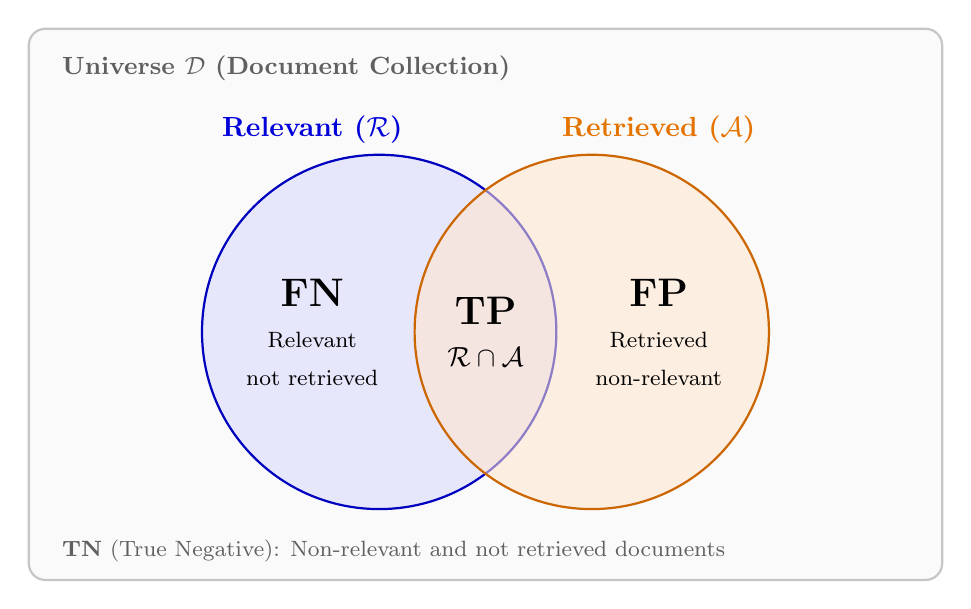
\begin{tikzpicture}
    % Document Collection Rectangle (Universe)
    \draw[thick, fill=gray!4, draw=gray!45, rounded corners=6pt] (-5.8, -3.3) rectangle (5.8, 3.7);
    \node[anchor=north west, font=\bfseries\small, text=gray!75!black] at (-5.5, 3.48) {Universe $\mathcal{D}$ (Document Collection)};

    % Circles (Relevant and Retrieved)
    \draw[thick, fill=blue!15, draw=blue!75!black, fill opacity=0.55] (-1.35, -0.15) circle (2.25cm);
    \draw[thick, fill=orange!20, draw=orange!80!black, fill opacity=0.55] (1.35, -0.15) circle (2.25cm);

    % Circle Set Titles (Above the circles with ample margin)
    \node[font=\bfseries\normalsize, blue!85!black] at (-2.2, 2.42) {Relevant ($\mathcal{R}$)};
    \node[font=\bfseries\normalsize, orange!90!black] at (2.2, 2.42) {Retrieved ($\mathcal{A}$)};

    % Region Labels (Centered and well-spaced)
    \node[align=center] at (-2.2, -0.15) {\textbf{\Large FN}\\[3pt]\footnotesize Relevant\\[1.5pt]\footnotesize not retrieved};
    \node[align=center] at (0, -0.15) {\textbf{\Large TP}\\[3pt]\normalsize $\mathcal{R} \cap \mathcal{A}$};
    \node[align=center] at (2.2, -0.15) {\textbf{\Large FP}\\[3pt]\footnotesize Retrieved\\[1.5pt]\footnotesize non-relevant};
    
    % True Negative label (Spacious bottom-left corner with ample clearance)
    \node[anchor=south west, font=\footnotesize, text=gray!75!black] at (-5.5, -3.2) {\textbf{TN} (True Negative): Non-relevant and not retrieved documents};
\end{tikzpicture}%
}
\caption{Set-theoretic Venn diagram of document retrieval and confusion regions.}
\label{fig:venn-retrieval-en}
\end{figure}

\subsection{Precision, Recall, and the Precision-Recall Trade-off}
\begin{definition}[Precision ($P$)]
The fraction of retrieved documents that are relevant:
\begin{equation}
P = \frac{TP}{TP + FP} = P(\text{relevant} \mid \text{retrieved})
\end{equation}
\end{definition}

\begin{definition}[Recall ($R$)]
The fraction of relevant documents in the collection that were successfully retrieved:
\begin{equation}
R = \frac{TP}{TP + FN} = P(\text{retrieved} \mid \text{relevant})
\end{equation}
\end{definition}

An inherent \textbf{trade-off} governs Precision and Recall:
\begin{itemize}
    \item Returning the entire document repository ($\text{Retrieved} = \mathcal{D}$) guarantees $R = 100\%$, but drops precision near zero ($P \approx 0$).
    \item Conversely, returning only the single most confident document can yield $P = 100\%$, at the expense of dismal recall.
\end{itemize}

\subsection{\texorpdfstring{The Harmonic Mean: F-Measure ($F_1$-Score)}{The Harmonic Mean: F-Measure (F1-Score)}}
To balance Precision and Recall into a single scalar metric that penalizes extreme disparity, the \textbf{F-Measure} calculates their \textbf{harmonic mean}:
\begin{equation}
F_1 = \frac{2}{\frac{1}{P} + \frac{1}{R}} = \frac{2 \cdot P \cdot R}{P + R} = \frac{2 \cdot TP}{2 \cdot TP + FP + FN}
\end{equation}

\begin{property}[Harmonic Mean Properties]
The harmonic mean exhibits key mathematical properties for evaluation:
\begin{enumerate}
    \item It is always upper-bounded by both the geometric and arithmetic means:
    \[
    \frac{2}{\frac{1}{a} + \frac{1}{b}} \le \sqrt{a \cdot b} \le \frac{a + b}{2}
    \]
    \item When the two operands diverge significantly, the harmonic mean is heavily drawn toward the \textbf{minimum} rather than the arithmetic average.
\end{enumerate}
\end{property}

\begin{example}[Edge Behavior of F-Measure]
Consider a degenerate retrieval system returning all documents: $R = 1.0$ and $P = 0.0001$.
\begin{itemize}
    \item The arithmetic mean yields an artificially inflated score:
    \[
    \frac{1.0 + 0.0001}{2} \approx 0.50 \quad (50\%)
    \]
    \item The harmonic mean ($F_1$) penalizes the system:
    \[
    F_1 = \frac{2 \cdot 1.0 \cdot 0.0001}{1.0 + 0.0001} \approx 0.0002 \quad (0.02\%)
    \]
\end{itemize}
This illustrates why the harmonic mean is mathematically favored over the arithmetic mean.
\end{example}

\subsection{\texorpdfstring{The Weighted $F_\beta$-Measure}{The Weighted F-beta Measure}}
When asymmetric priority is given to Precision versus Recall, a weighting parameter $\alpha \in [0, 1]$ is introduced:
\begin{equation}
F = \frac{1}{\alpha \frac{1}{P} + (1 - \alpha) \frac{1}{R}}
\end{equation}
Setting $\alpha = \frac{1}{1 + \beta^2}$ leads to the standard \textbf{$F_\beta$} formulation:
\begin{equation}
F_\beta = \frac{(1 + \beta^2) \cdot P \cdot R}{\beta^2 \cdot P + R}
\end{equation}
\begin{itemize}
    \item Values of $\beta < 1$ (e.g., $\beta = 0.5$) emphasize \textbf{Precision} over Recall (favored in Web search).
    \item Values of $\beta > 1$ (e.g., $\beta = 2.0$) emphasize \textbf{Recall} over Precision (crucial in legal discovery, patent search, and clinical meta-analyses).
\end{itemize}

\FloatBarrier
\section{Rank-Based Measures (Binary Relevance)}

Modern search engines return ranked lists ordered by descending relevance scores. Furthermore, Web users rarely look beyond the first page of results ($k = 10$ or $k = 30$).

\subsection{\texorpdfstring{Precision@k ($P@k$) and Recall@k ($R@k$)}{Precision@k and Recall@k}}
\begin{definition}[Precision@k]
Given a fixed rank cutoff $k \in \mathbb{N}^+$, Precision@k is the fraction of relevant documents within the top $k$ positions:
\begin{equation}
P@k = \frac{1}{k} \sum_{i=1}^k \mathrm{rel}_i
\end{equation}
where $\mathrm{rel}_i \in \{0, 1\}$ represents the binary relevance of the document at rank $i$.
\end{definition}

\begin{example}[Computing Precision@k]
Consider a ranked list with binary relevance sequence for the top 5 positions $\langle 1, 1, 0, 0, 1 \rangle$:
\begin{itemize}
    \item $P@1 = \frac{1}{1} = 1.00$
    \item $P@2 = \frac{2}{2} = 1.00$
    \item $P@3 = \frac{2}{3} \approx 0.66$
    \item $P@4 = \frac{2}{4} = 0.50$ (note that $P@4 < P@3$)
    \item $P@5 = \frac{3}{5} = 0.60$
\end{itemize}
\end{example}

\begin{alertblock}{The Distortion of $P@k$ When Averaged Across Queries}
While $P@k$ is intuitive for estimating top-page result quality, it suffers from a critical methodological flaw when averaged across heterogeneous queries:
\begin{itemize}
    \item If a specific query $q_A$ possesses only $R_A = 2$ relevant documents in the entire corpus, the theoretical maximum possible $P@10(q_A)$ is capped at $\frac{2}{10} = 0.20$, even if a flawless engine places both relevant documents at ranks 1 and 2!
    \item Averaging raw $P@10$ across queries penalizes the retrieval engine for the intrinsic scarcity of relevant documents for specific information needs, rather than algorithmic ranking errors.
\end{itemize}
Similarly, the complementary measure $Recall@k$ ($R@k$) evaluates the fraction of all relevant documents recovered within rank $k$:
\begin{equation}
Recall@k = \frac{1}{R} \sum_{i=1}^k \mathrm{rel}_i
\end{equation}
\end{alertblock}

\subsection{Average Precision (AP)}
\textbf{Average Precision} (AP) summarizes the entire Precision-Recall curve into a single scalar score for a given query, evaluating instantaneous precision at each rank position where recall increases.

\begin{definition}[Average Precision]
For a ranking of $N$ documents corresponding to a query with $R$ total relevant documents in the collection:
\begin{equation}
AP = \frac{1}{R} \sum_{k=1}^N P@k \cdot \mathrm{rel}_k
\end{equation}
\end{definition}

\begin{property}[Geometric Interpretation and the Role of $1/R$]
Average Precision carries a direct analytical meaning:
\begin{enumerate}
    \item Each time a relevant document is encountered at rank $k$, recall increases by a discrete increment $\Delta Recall = \frac{1}{R}$. AP accumulates the rectangular areas $P@k \cdot \Delta Recall$, representing the \textbf{discrete numerical approximation of the Area Under the Precision-Recall Curve} (AUC-PR).
    \item Normalizing by $R$ (the total number of relevant documents in the corpus) ensures that relevant documents omitted from the top-$N$ candidate pool implicitly contribute zero precision, heavily penalizing systems with incomplete recall.
\end{enumerate}
\end{property}

\begin{figure}[htbp]
\centering
\begin{tikzpicture}[
    scale=0.85,
    docrel/.style={rectangle, rounded corners=2pt, draw=teal!80!black, fill=teal!20, thick, minimum width=1.1cm, minimum height=0.65cm, font=\footnotesize\bfseries},
    docnon/.style={rectangle, rounded corners=2pt, draw=red!70!black, fill=red!10, thick, minimum width=1.1cm, minimum height=0.65cm, font=\footnotesize},
    lbl/.style={font=\scriptsize, align=center}
]
    % Document ranking blocks
    \node[lbl] at (-1.5, 0.35) {Rank Position ($k$):};
    \node[lbl] at (-1.5, -0.35) {Document:};
    \node[lbl] at (-1.5, -1.05) {Precision@k:};

    \foreach \k/\rel/\p/\type in {
        1/1/1.00/docrel,
        2/0/---/docnon,
        3/1/0.67/docrel,
        4/0/---/docnon,
        5/1/0.60/docrel%
    } {
        \node[font=\footnotesize\bfseries] at (\k*1.6, 0.35) {$k=\k$};
        \node[\type] (b\k) at (\k*1.6, -0.35) {\ifnum\rel=1 Rel\else NonRel\fi};
        \node[font=\footnotesize] at (\k*1.6, -1.05) {\ifnum\rel=1 \textbf{\p}\else \color{gray!60}--- \fi};
    }

    \draw[-Stealth, thick, blue!80!black] (0.5, 0.7) -- node[above, font=\scriptsize] {Search Engine Output Order} (8.5, 0.7);
\end{tikzpicture}
\caption{Schematic representation of Average Precision calculation over 5 documents with $R=3$ total relevant items.}
\label{fig:ap-blocks-en}
\end{figure}

\begin{example}[Basic Calculation with $R=3$ Relevant Documents]
Consider the ranking scenario in Figure~\ref{fig:ap-blocks-en} with $R=3$ total relevant documents appearing at ranks $k_1 = 1$, $k_2 = 3$, and $k_3 = 5$:
\[
P@1 = \frac{1}{1} = 1.00, \quad P@3 = \frac{2}{3} \approx 0.667, \quad P@5 = \frac{3}{5} = 0.60
\]
The resulting Average Precision is:
\begin{equation}
AP = \frac{1}{3} \left( 1.00 + \frac{2}{3} + \frac{3}{5} \right) = \frac{1}{3} \left( 2.267 \right) \approx 0.756 \quad (75.6\%)
\end{equation}
\end{example}

\begin{example}[Comparative Analysis Between Two Rankings]
Consider a query associated with $R = 6$ relevant documents in the collection. Two competing search algorithms output the following top-10 ranked results:
\begin{itemize}
    \item \textbf{Ranking \#1:} Relevant items concentrated early in the list:
    \[
    \langle \text{Rel}, \text{NonRel}, \text{Rel}, \text{Rel}, \text{Rel}, \text{Rel}, \text{NonRel}, \text{NonRel}, \text{NonRel}, \text{Rel} \rangle
    \]
    \item \textbf{Ranking \#2:} Relevant items delayed and scattered:
    \[
    \langle \text{NonRel}, \text{Rel}, \text{NonRel}, \text{NonRel}, \text{Rel}, \text{Rel}, \text{Rel}, \text{NonRel}, \text{Rel}, \text{Rel} \rangle
    \]
\end{itemize}
Table~\ref{tab:ap-comparison-en} presents the step-by-step evolution of Precision and Recall across all 10 ranks.

\begin{table}[htbp]
\centering
\resizebox{\textwidth}{!}{%
\begin{tabular}{c c c c c c c}
\toprule
& \multicolumn{3}{c}{\textbf{Ranking \#1}} & \multicolumn{3}{c}{\textbf{Ranking \#2}} \\
\cmidrule(lr){2-4} \cmidrule(lr){5-7}
\textbf{Rank ($k$)} & \textbf{Item} & \textbf{Recall} & \textbf{Precision} & \textbf{Item} & \textbf{Recall} & \textbf{Precision} \\
\midrule
1  & \textbf{Rel}    & 0.17 & \textbf{1.00} & NonRel          & 0.00 & --- \\
2  & NonRel          & 0.17 & ---           & \textbf{Rel}    & 0.17 & \textbf{0.50} \\
3  & \textbf{Rel}    & 0.33 & \textbf{0.67} & NonRel          & 0.17 & --- \\
4  & \textbf{Rel}    & 0.50 & \textbf{0.75} & NonRel          & 0.17 & --- \\
5  & \textbf{Rel}    & 0.67 & \textbf{0.80} & \textbf{Rel}    & 0.33 & \textbf{0.40} \\
6  & \textbf{Rel}    & 0.83 & \textbf{0.83} & \textbf{Rel}    & 0.50 & \textbf{0.50} \\
7  & NonRel          & 0.83 & ---           & \textbf{Rel}    & 0.67 & \textbf{0.57} \\
8  & NonRel          & 0.83 & ---           & NonRel          & 0.67 & --- \\
9  & NonRel          & 0.83 & ---           & \textbf{Rel}    & 0.83 & \textbf{0.56} \\
10 & \textbf{Rel}    & 1.00 & \textbf{0.60} & \textbf{Rel}    & 1.00 & \textbf{0.60} \\
\midrule
\multicolumn{2}{l}{\textbf{Average Precision (AP)}} & & \textbf{0.78} & & & \textbf{0.52} \\
\bottomrule
\end{tabular}%
}
\caption{Detailed comparative evaluation of Average Precision between Ranking \#1 and Ranking \#2.}
\label{tab:ap-comparison-en}
\end{table}

The resulting AP scores evaluate to:
\begin{align*}
AP(\text{Ranking \#1}) &= \frac{1.00 + 0.67 + 0.75 + 0.80 + 0.83 + 0.60}{6} = \frac{4.65}{6} \approx \mathbf{0.78} \\
AP(\text{Ranking \#2}) &= \frac{0.50 + 0.40 + 0.50 + 0.57 + 0.56 + 0.60}{6} = \frac{3.13}{6} \approx \mathbf{0.52}
\end{align*}
Although both systems achieve identical overall recall ($R = 100\%$ across 10 retrieved documents), Ranking \#1 obtains a substantially higher score ($0.78$ vs $0.52$) because it rewards front-loading relevant items.
\end{example}

\subsection{Mean Average Precision (MAP)}
To quantify overall effectiveness across a suite of $|\mathcal{Q}|$ benchmark queries, we compute the arithmetic mean of their respective AP scores:

\begin{definition}[Mean Average Precision]
\begin{equation}
MAP = \frac{1}{|\mathcal{Q}|} \sum_{q \in \mathcal{Q}} AP(q)
\end{equation}
\end{definition}

\begin{property}[Macro-Averaging vs. Micro-Averaging]
MAP formally implements a \textbf{Macro-Averaging} scheme: each query carries identical statistical weight $1/|\mathcal{Q}|$.
\begin{itemize}
    \item In contrast, \textit{Micro-Averaging} (pooling all instantaneous precisions across all queries and dividing by the total sum of relevant documents) would be overwhelmingly dominated by a handful of broad queries (e.g., \texttt{``movies''} or \texttt{``news''}, which often match thousands of relevant documents), drowning out performance on specific long-tail queries.
    \item Macro-Averaging ensures that every individual information need receives equal representation in the final benchmark metric.
\end{itemize}
\end{property}

\begin{example}[Computing MAP Over Two Queries]
Consider an evaluation suite consisting of two distinct queries $q_1$ and $q_2$:
\begin{itemize}
    \item \textbf{Query 1 ($R_1 = 5$ total relevant documents):} The engine returns 5 relevant items at ranks $k \in \{1, 3, 6, 9, 10\}$ with precisions $1.00$, $0.67$, $0.50$, $0.44$, and $0.50$:
    \[
    AP(q_1) = \frac{1.00 + 0.67 + 0.50 + 0.44 + 0.50}{5} = \frac{3.11}{5} \approx \mathbf{0.62}
    \]
    \item \textbf{Query 2 ($R_2 = 3$ total relevant documents):} The engine returns 3 relevant items at ranks $k \in \{2, 5, 7\}$ with precisions $0.50$, $0.40$, and $0.43$:
    \[
    AP(q_2) = \frac{0.50 + 0.40 + 0.43}{3} = \frac{1.33}{3} \approx \mathbf{0.44}
    \]
\end{itemize}
The overall Mean Average Precision across both queries is:
\begin{equation}
MAP = \frac{AP(q_1) + AP(q_2)}{2} = \frac{0.62 + 0.44}{2} = \mathbf{0.53}
\end{equation}
\end{example}

\subsection{Truncated Ranking Measures: AP@k and MAP@k}
In Web search and Recommender Systems, evaluating AP across an entire collection is impractical (the true total count $R$ of relevant items is unknown) and disconnected from user browsing habits.
Engines thus adopt rank-truncated formulations (\textbf{MAP@K}):

\begin{definition}[AP@K and MAP@K]
Given a fixed rank cutoff $K$ (typically $K=10$ or $K=20$), Average Precision at $K$ for query $q_i$ is defined as:
\begin{equation}
AP@K(q_i) = \frac{1}{K_i} \sum_{k=1}^K P@k(q_i) \cdot \mathrm{rel}(q_i, k)
\end{equation}
where the normalizing denominator $K_i$ reflects the number of relevant items within the top $K$:
\begin{equation}
K_i = \sum_{k=1}^K \mathrm{rel}(q_i, k) \quad \left(\text{or } K_i = \min(R_i, K)\right)
\end{equation}
The global \textbf{MAP@K} across query suite $\mathcal{Q}$ evaluates to:
\begin{equation}
MAP@K(\mathcal{Q}) = \frac{1}{|\mathcal{Q}|} \sum_{q_i \in \mathcal{Q}} AP@K(q_i)
\end{equation}
\end{definition}
This formulation resolves the fundamental flaw of raw $P@K$: by normalizing by $K_i$ instead of a rigid $K$, a query with only 2 relevant documents that places both in the top 2 slots attains $AP@10 = 1.0$ rather than being artificially capped at $0.20$.

\subsection{Mean Reciprocal Rank (MRR)}
In tasks such as known-item search, navigational queries (e.g., locating an institutional homepage), or factoid retrieval, the user is interested solely in finding the \textbf{first correct document}. User effort is inversely proportional to the rank of that first hit:

\begin{definition}[Reciprocal Rank and MRR]
Let $\mathrm{rank}_1(q)$ denote the rank position of the first relevant document returned for query $q$. The \textbf{Reciprocal Rank} (RR) is:
\begin{equation}
RR(q) = \frac{1}{\mathrm{rank}_1(q)}
\end{equation}
The \textbf{Mean Reciprocal Rank} (MRR) across all queries is:
\begin{equation}
MRR = \frac{1}{|\mathcal{Q}|} \sum_{q \in \mathcal{Q}} \frac{1}{\mathrm{rank}_1(q)}
\end{equation}
\end{definition}
If the first relevant hit appears at rank 1, the score is $1.0$; if at rank 2, it drops to $0.5$; if delayed to rank 10, it falls to $0.1$.

\FloatBarrier
\section{Beyond Binary Relevance: Graded Relevance and NDCG}

In practical Web and commercial applications, binary judgments prove inadequate. Consider the following real-world Google search query:
\begin{center}
\texttt{Query: ``information retrieval unipi''}
\end{center}
A commercial SERP returns pages exhibiting distinct qualitative levels of utility:
\begin{enumerate}
    \item \textbf{Course DidaWiki (Instructor, CFU, syllabus, lecture notes):} The primary resource fully satisfying user search intent $\implies$ \textbf{Highly Relevant ($r = 3$)}.
    \item \textbf{Official UniPi Valutami Portal (Exam registration and administrative syllabus):} Authoritative institutional record but lacks study material $\implies$ \textbf{Relevant ($r = 2$)}.
    \item \textbf{Master's Degree PDF Brochure:} Contains only a brief mention of the course $\implies$ \textbf{Marginally Relevant ($r = 1$)}.
    \item \textbf{Unrelated articles or campus news:} $\implies$ \textbf{Irrelevant ($r = 0$)}.
\end{enumerate}
While all top three pages are pertinent, user satisfaction depends heavily on displaying the most informative page at rank 1. To capture this nuance, IR formalizes multi-grade relevance scales ($r \in \{0, 1, 2, 3\}$ or $\{0, \dots, 4\}$).

The \textbf{Discounted Cumulative Gain} (DCG) framework, introduced by J\"arvelin and Kek\"al\"ainen~\cite{jarvelin2002}, rests on two assumptions:
\begin{enumerate}
    \item Highly relevant documents are much more useful than marginally relevant ones.
    \item The lower a document appears in the ranking, the less likely the user is to examine it; hence, gain must be discounted with descending rank.
\end{enumerate}

\subsection{Cumulative Gain (CG) and Discounted Cumulative Gain (DCG)}
\begin{definition}[Cumulative Gain at Rank $p$]
Given a vector of graded relevance values $\mathbf{r} = [r_1, r_2, \dots, r_p]$, the Cumulative Gain is the unweighted sum:
\begin{equation}
CG_p = \sum_{i=1}^p r_i
\end{equation}
$CG_p$ is position-insensitive: swapping a highly relevant document at rank 1 with one at rank 10 leaves $CG_p$ unchanged.
\end{definition}

\begin{definition}[Discounted Cumulative Gain (Standard Formulation)]
Standard DCG applies a logarithmic discount based on rank $i$:
\begin{equation}
DCG_p = r_1 + \sum_{i=2}^p \frac{r_i}{\log_2(i)}
\label{eq:dcg-standard-en}
\end{equation}
\end{definition}

\begin{alertblock}{Behavioral Meaning of the Logarithmic Discount}
The discount factor $\frac{1}{\log_2(i)}$ reflects the exponential decay of user visual attention under cascade reading models:
\begin{itemize}
    \item At rank $i = 4$, the discount factor is $\frac{1}{\log_2(4)} = \frac{1}{2}$: perceived informative utility is cut in half relative to rank 1.
    \item At rank $i = 8$, the factor drops to $\frac{1}{\log_2(8)} = \frac{1}{3}$.
    \item At rank $i = 16$, the factor falls to $\frac{1}{\log_2(16)} = \frac{1}{4}$.
\end{itemize}
\end{alertblock}

Commercial search engines (Google, Bing) frequently utilize the \textbf{exponential formulation}:
\begin{equation}
DCG_p^{\text{exp}} = \sum_{i=1}^p \frac{2^{r_i} - 1}{\log_2(i + 1)}
\label{eq:dcg-exp-en}
\end{equation}
\begin{noteblock}{Summation Index Clarification}
Note the index shift in the logarithm denominator:
\begin{itemize}
    \item In Equation~\eqref{eq:dcg-standard-en}, $r_1$ is separated to prevent division by $\log_2(1) = 0$, while the summation starts at $i=2$ with $\log_2(i)$.
    \item In Equation~\eqref{eq:dcg-exp-en}, the summation starts directly at $i=1$ by taking $\log_2(i+1)$ ($\log_2(1+1) = \log_2(2) = 1$).
    \item Furthermore, numerator $2^{r_i} - 1$ non-linearly rewards top-tier relevance ($r=3 \implies 2^3 - 1 = 7$, vs. $r=1 \implies 2^1 - 1 = 1$), severely penalizing any demotion of stellar results.
\end{itemize}
\end{noteblock}

\subsection{Normalized Discounted Cumulative Gain}
Because different queries have varying numbers of relevant documents, raw $DCG_p$ scores cannot be compared across queries. We normalize by the \textbf{Ideal DCG} ($IDCG_p$), obtained by computing the DCG of the ideal ranking sorted by relevance descending:
\begin{equation}
NDCG_p = \frac{DCG_p}{IDCG_p} \quad \in [0, 1]
\end{equation}

\subsection{Complete Numerical Walkthrough}
Consider the following 10-document ranking, judged on a scale of $0$--$3$:
\[
\mathbf{r} = [3, \, 2, \, 3, \, 0, \, 0, \, 1, \, 2, \, 2, \, 3, \, 0]
\]
The ideal sorted ranking is:
\[
\mathbf{r}^* = [3, \, 3, \, 3, \, 2, \, 2, \, 2, \, 1, \, 0, \, 0, \, 0]
\]
Table~\ref{tab:ndcg-step-by-step-en} summarizes the step-by-step progression across all 10 ranks.

\begin{table}[htbp]
\centering
\resizebox{\textwidth}{!}{%
\begin{tabular}{c c l c >{\bfseries}c c c >{\bfseries}c >{\bfseries}c}
\toprule
$i$ & $r_i$ & Discount & Discounted Gain & $DCG@i$ & $r_i^*$ & Ideal Gain & $IDCG@i$ & $NDCG@i$ \\
\midrule
1 & 3 & 1.000 & 3.00 & 3.00 & 3 & 3.00 & 3.00 & 1.00 \\
2 & 2 & $\log_2(2) = 1.000$ & 2.00 & 5.00 & 3 & 3.00 & 6.00 & 0.83 \\
3 & 3 & $\log_2(3) = 1.585$ & 1.89 & 6.89 & 3 & 1.89 & 7.89 & 0.87 \\
4 & 0 & $\log_2(4) = 2.000$ & 0.00 & 6.89 & 2 & 1.00 & 8.89 & 0.76 \\
5 & 0 & $\log_2(5) = 2.322$ & 0.00 & 6.89 & 2 & 0.86 & 9.75 & 0.71 \\
6 & 1 & $\log_2(6) = 2.585$ & 0.39 & 7.28 & 2 & 0.77 & 10.52 & 0.69 \\
7 & 2 & $\log_2(7) = 2.807$ & 0.71 & 7.99 & 1 & 0.36 & 10.88 & 0.73 \\
8 & 2 & $\log_2(8) = 3.000$ & 0.67 & 8.66 & 0 & 0.00 & 10.88 & 0.80 \\
9 & 3 & $\log_2(9) = 3.170$ & 0.95 & 9.61 & 0 & 0.00 & 10.88 & 0.88 \\
10 & 0 & $\log_2(10) = 3.322$ & 0.00 & 9.61 & 0 & 0.00 & 10.88 & 0.88 \\
\bottomrule
\end{tabular}%
}
\caption{Detailed trace of $DCG@i$, $IDCG@i$, and $NDCG@i$ computation for ranks $1$ through $10$.}
\label{tab:ndcg-step-by-step-en}
\end{table}

\subsection{Comparing Alternative Ranking Functions}
Consider 4 documents $\{d_1, d_2, d_3, d_4\}$ with graded assessments:
\[
r(d_1) = 0, \quad r(d_2) = 1, \quad r(d_3) = 2, \quad r(d_4) = 2
\]
\begin{itemize}
    \item \textbf{Ground Truth ($GT$):} Ordering $\langle d_4, d_3, d_2, d_1 \rangle$ with relevance vector $[2, 2, 1, 0]$:
    \begin{align*}
    IDCG_4 &= 2 + \frac{2}{\log_2(2)} + \frac{1}{\log_2(3)} + 0 = 2 + 2 + 0.6309 = 4.6309 \\
    NDCG_{GT} &= 1.00
    \end{align*}
    \item \textbf{Ranking Function 1 ($RF_1$):} Ordering $\langle d_3, d_4, d_2, d_1 \rangle$ with relevance $[2, 2, 1, 0]$.
    Because the first two documents share identical relevance ($r=2$), their permutation incurs no positional penalty:
    \begin{align*}
    DCG_{RF_1} &= 2 + \frac{2}{\log_2(2)} + \frac{1}{\log_2(3)} = 4.6309 \\
    NDCG_{RF_1} &= \frac{4.6309}{4.6309} = 1.00
    \end{align*}
    \item \textbf{Ranking Function 2 ($RF_2$):} Ordering $\langle d_3, d_2, d_4, d_1 \rangle$ with relevance $[2, 1, 2, 0]$.
    Here, $d_2$ ($r=1$) erroneously outranks $d_4$ ($r=2$):
    \begin{align*}
    DCG_{RF_2} &= 2 + \frac{1}{\log_2(2)} + \frac{2}{\log_2(3)} + 0 = 2 + 1 + 1.2619 = 4.2619 \\
    NDCG_{RF_2} &= \frac{DCG_{RF_2}}{IDCG_4} = \frac{4.2619}{4.6309} \approx 0.9203
    \end{align*}
\end{itemize}
This illustrates how NDCG mathematically penalizes rank inversions in direct proportion to the relevance difference.
